\documentclass[11pt]{article}
\usepackage[utf8]{inputenc}
\usepackage{amsmath}
\usepackage{amsfonts}
\usepackage{amssymb}
\usepackage{graphicx}
\usepackage[super]{nth}
\usepackage{amsthm}
\newtheorem{theorem}{Theorem}
\newtheorem{objective}{Objective}
\newtheorem{procedure}{Procedure}
\newtheorem{model}{Model}


\makeatletter
\renewcommand{\maketitle}{
\begin{center}

\pagestyle{empty}
\phantom{.}  %necessary to add space on top before the title
\vspace{3cm}

{\Huge \bf \@title\par}
\vspace{2.5cm}

{\LARGE Marcel Gietzmann-Sanders}\\[1cm]

{\Large\@date}

\vspace{2.5cm}
{\Large Dr. Andrew Seitz}\hspace{2cm}{\Large Dr. Curry Cunningham}\\[2cm]{\Large Michael Courtney, M.S.}\\[2cm]
College of Fisheries and Ocean Sciences\\
University of Alaska Fairbanks


\end{center}
}\makeatother


\title{Spatio-Temporal Modeling and Simulation}

\date{2024}
\setcounter{tocdepth}{2}
\begin{document}
\maketitle
\newpage
\tableofcontents
\newpage

\section{Log Odds Modeling}

\begin{objective}
To provide tooling that allows for using machine learning methods to fit models of the form

$$\psi_k = G(\eta_k)$$

that maximize the following objective:


$$\mathcal{L}=\prod_i P'(v_i | \eta_i)$$

where:

$$P'(v_i|\eta_i) = \frac{e^{\psi_i}}{\sum_k e^{\psi_k}}$$

These models will be known as log odds models as they predict the "log odds for" each outcome $v_k$ given the information contained in $\eta_k$. 

\end{objective}

\subsection{Fitting an Odds Model}

Our objective in using machine learning (ML) is to reduce the time spent looking for the particular form of $G(\eta_k)$ by instead allowing that form to be fit given the data at hand. Deep Learning (DL) models are especially well suited to this problem as they are both parametric (see Section \ref{convergence issues} for why non-parametric models are not well suited to our problem) and have been shown to be able to represent just about any function given a large enough network \cite{LiquetMokaNazarathy2024DeepLearning}. There is also a robust field around probabilistic deep learning that, as we shall see in a moment, we can take advantage of \cite{durr}.
\newline

Taking a look at traditional probabilistic classifiers we can see that they have two things in common with our intended log odds modeling. 

First, probabilistic classifiers use the categorical cross entropy cost function to optimize their weights. This cost function happens to be just another name for optimizing for the Log Likelihood of the data \cite{durr}. Therefore probabilistic DL shares the same objective function as we do.

Second, the final layer in a probabilistic DL network is the one that produces a probability for each class. This layer uses the softmax function as it's activation function which if if $a_i=W_i x+b_i$ is given by - $\frac{e^{a_i}}{\sum_k e^{a_k}}$. This means that if we can get our $\psi_k$ to be the $a_i$ that we'll be, in effect, training a log odds model.

We can do this by taking advantage of Keras' Functional API \cite{kerasfunctional} which allows us to split our network into a branches and also share layers between branches. Specifically we can follow the following steps:

\begin{enumerate}
\item Define a series of layers that represent our underlying log odds model (these layers should end in a layer of output size 1 which will represent our $\psi_k$).
\item Split our training decisions into $N$ choices.
\item Create a branch in our overall model for each of these $N$ choices.
\item Converge the branches at a softmax layer where the weights are the identity matrix $I$ and the biases all 0 (this ensures we directly pass through our $\psi_k$ to the softmax function).
\item Use categorical cross entropy as our fitness function.
\end{enumerate}

This architecture is illustrated by Fig. \ref{fig:logarch}.

\begin{figure}[h!] 
  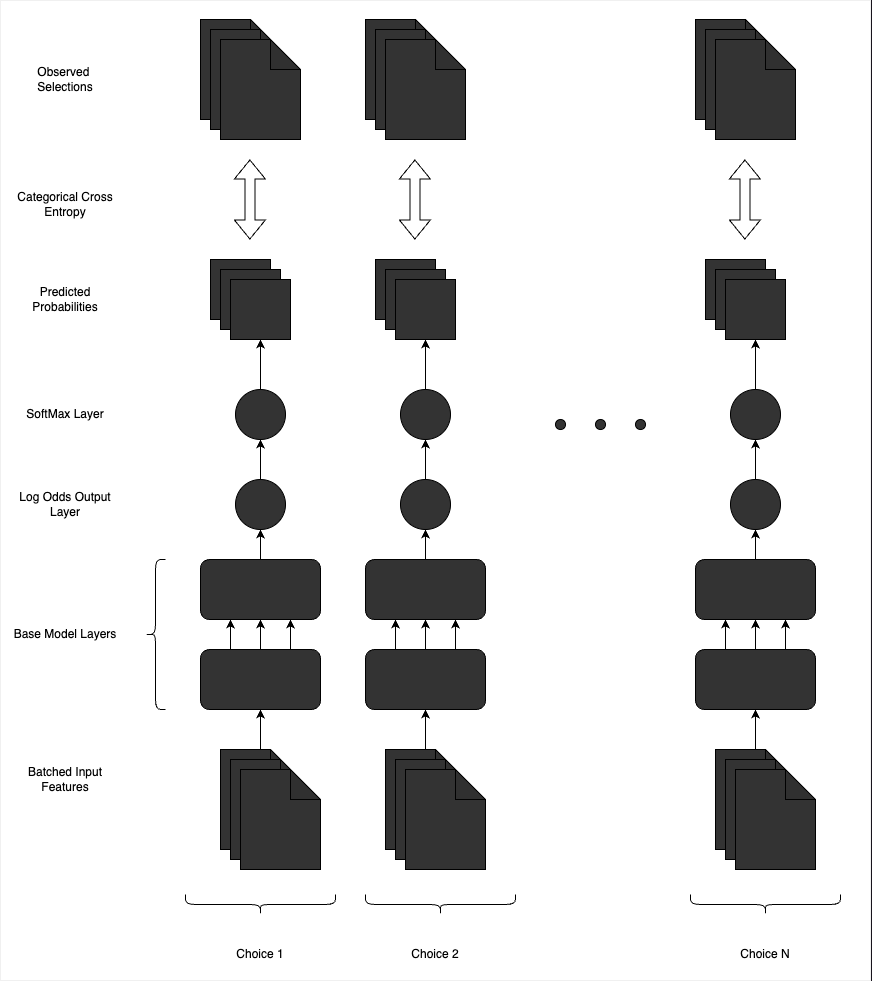
\includegraphics[width=\linewidth]{logarch.png}
  \caption{Overall Architecture}
  \label{fig:logarch}
\end{figure}

The main advantage of this architecture as opposed to a more classic approach to probabilistic DL is the fact that the weights are shared on each of the branches. This has the effect of drastically reducing the number of parameters in our network meaning that we can use far less data to train this model then we'd need to train a full bore, fully connected, probabilistic model. Each of our columns in Fig. \ref{fig:logarch} is in fact the same model and therefore updates coming from each of the columns goes to all of the columns.

This, then, solves one of our issues - reducing the variance in the model by switching to the log odds approach. But the other issue we're trying to solve is being able to predict on variable numbers of choices per decision. How does that work out here?\newline

Well, in the case of training we know the maximum number of choices in any of our training decisions. Therefore we can set $N$ to this maximum and for decisions where we have fewer than $N$ choices we can simply provide some kind of default "do not choose" feature for the "missing" choices. 

Later during inference on new data we can simply take our shared layers and use them to predict on each of the choices we're presented with. Just another demonstration that while we're using the architecture in Fig. \ref{fig:logarch} in order to \textit{train} the log odds model, the actual log odds model is simply the shared layers in a single column behind the softmax layer. 


\newpage
\section{Appendices}

\subsection{Convergence Issue with Non-Parametric Log Odds Models} \label{convergence issues}

All standard Machine Learning (ML) pipelines assume that you have at least two things - targets and features. In our case we certainly have the latter but our target $\psi_k$ is both unknown to us and also unmeasureable. So how are we to fit ML models if we have no target? In short, through iteration. Let's see how this can be done.\newline

First some notation to help us. Our data is composed of a series of decisions $D_j=\lbrace v_{jk} \rbrace$ where $j$ indicates each of the specific decisions and $k$ the options within each decision. For each iteration we will build a model $\hat{G_i}(\eta_{jk})$ using the pairs $\psi_{jk(i-1)},\eta_{jk}$. We will designate the outcome of that model $\phi_{jki}$:

$$\phi_{jki} = \hat{G_i}(\eta_{jk})$$

Our probability is therefore:

$$P_i'(v_{jk}|\eta_{jk})=\frac{e^{\phi_{jki}}}{\sum_p e^{\phi_{jpi}}}$$

Now if the $k$ selected per decision $D_j$ is given by $s_j$ we want to maximize:

$$\mathcal{L}=\prod_j P_i'(v_{js_j} | \eta_{js_j})\rightarrow \sum_j \ln{\left[ P_i'(v_{js_j} | \eta_{js_j}) \right]}$$

Using this information we will then propose an update $u_{jki}$ s.t. $\psi_{jki}=\phi_{jki} + u_{jki}$ and repeat our iteration loop. 

With that notation cleared up we can begin our iteration procedure. \newline

First, let's assume we already have a guess for $\psi_{jk(i-1)}$. We can therefore train our model off of the $\psi_{jk0},\eta_{jk}$ pairs in standard ML fashion. Specifically we will fit a model that optimizes Mean Squared Error (the most common objective across ML software packages):

$$\min{\left[ \sum_{jk}\left(\hat{G_i}(\eta_{jk}) - \psi_{jk(i-1)}\right)^2 \right]}$$

We now need to choose a set of updates $u_{jki}$. To get these we will turn to our overall objective function:

$$\sum_j \ln{\left[ P_i'(v_{js_j} | \eta_{js_j}) \right]}= \sum_j \ln{\left[ \frac{e^{\phi_{js_ji}}}{\sum_p e^{\phi_{jpi}}} \right]}$$

Let's look at the gradient of this w.r.t the $\phi_{jki}$. There are two cases:

$$\partial_{\phi_{js_ji}}\ln{\mathcal{L}}
=
\frac{1}{P_i'(v_{js_j} | \eta_{js_j})}\frac{\sum_p e^{\phi_{jpi}}-e^{\phi_{js_ji}}}{\left( \sum_p e^{\phi_{jpi}} \right)^2} e^{\phi_{js_ji}}
=
1-P_i'(v_{js_j} | \eta_{js_j}) $$ 

$$\partial_{\phi_{j\not{s_j}i}}\ln{\mathcal{L}}
=
\frac{1}{P_i'(v_{js_j} | \eta_{js_j})}\frac{-e^{\phi_{js_ji}}}{\left( \sum_p e^{\phi_{jpi}} \right)^2} e^{\phi_{j\not{s_j}i}}
= 
-P_i'(v_{j\not{s_j}} | \eta_{j\not{s_j}})$$ 

Next for point of illustration let's suppose that there are a set of $\psi_{jki}$ which we'll designate as $Z$ which share the same features $\eta$, i.e. our model has to give a single $\phi_{jki}$ for all such options. Our derivative then for that collection $Z$ is given by:

$$\partial_Z \ln{\mathcal{L}}=\sum_{\phi_{js_ji} \in Z}\left(1-P_i'(v_{js_j} | \eta_{js_j}) \right)-\sum_{\phi_{j\not{s_j}i}\in Z}P_i'(v_{j\not{s_j}} | \eta_{j\not{s_j}})$$

Given classic optimization tactics we know that our function will be maximized when these sums are $0$ (and technically we'd also want to know that the second derivative was negative but we'll assume that's the case given how our iterations will work). \newline

With this in mind let's now propose that our updates are given by:

$$u_{jki} = \alpha_i \partial_{\phi_{jki}} \ln{\mathcal{L}} $$

where $\alpha_i$ is a constant we'll call our "learning rate". Note that by using this update we will increase our $\psi_{jki}$ guess where it corresponds to a taken option ($s_j$) and will decrease it where it corresponds to an option not taken ($\not{s_j}$). This will therefore push us towards maximizing $\ln{\mathcal{L}}$ as opposed to minimizing it. \newline

We are left with a final question - will our iteration sequence end when we've found the maximizing guesses of $\psi_{jki}$? To answer this we turn back to the term we are maximizing when fitting the $\hat{G_i}$: 

$$\min{\left[ \sum_{jk}\left(\hat{G_i}(\eta_{jk}) - \psi_{jk(i-1)}\right)^2 \right]}$$

Our new fit will look like:

$$\sum_{jk}\left(\hat{G}_{i+1}(\eta_{jk}) - (\hat{G}_i(\eta_{jk}) + u_{jki})\right)^2=\sum_{jk}\left( \delta \hat{G}_{jk} - u_{jki}\right)^2$$

Given our $Z$ once again we can take the derivative w.r.t $\delta \hat{G}_{jk}$ where $\phi_{jki} \in Z$. 

$$\partial_Z \left[ \sum_{jk}\left( \delta \hat{G} - u_{jki}\right)^2 \right] = \sum_{\phi_{jki} \in Z} 2\left( \delta \hat{G} - u_{jki}\right) = 2\sum_{\phi_{jki} \in Z} \delta \hat{G} - 2\sum_{\phi_{jki} \in Z} u_{jki}$$

But now remember that if we've maximized w.r.t $Z$ that:

$$\sum_{\phi_{jki} \in Z} u_{jki} = 0$$

which means that in order for our partial derivative above to be zero (and therefore our error term be at a minimum) that $\delta \hat{G}=0$. And this means our iteration will have stopped! 

\newpage

\begin{procedure}{Fitting a Log Odds Model}
\begin{enumerate}
\item Collect decisions $D_j$ and corresponding features $\eta_{jk}$, options $v_{jk}$, and selection $s_j$. 
\item Make an initial guess $\psi_{jk0} = 0$.
\item Fit $\hat{G}_i$ on the pairs of $\psi_{jk(i-1)},\eta_{jk}$ using MSE to produce the $\phi_{jki}$.
\item Generate the $u_{jki} = \alpha_i \partial_{\phi_{jki}} \ln{\mathcal{L}}$ and produce a new set of $\psi_{jki}$.
\item Repeat 3 and 4 until, varying $\alpha_i$ until convergence. 

$$\partial_{\phi_{js_ji}}\ln{\mathcal{L}}=1-P_i'(v_{js_j} | \eta_{js_j})$$ 

$$\partial_{\phi_{j\not{s_j}i}}\ln{\mathcal{L}}=-P_i'(v_{j\not{s_j}} | \eta_{j\not{s_j}})$$ 
\end{enumerate}

\end{procedure}

There is however an issue with this approach. Recall that our gradient is:

$$\partial_Z \ln{\mathcal{L}}=\sum_{\phi_{js_ji} \in Z}\left(1-P_i'(v_{js_j} | \eta_{js_j}) \right)-\sum_{\phi_{j\not{s_j}i}\in Z}P_i'(v_{j\not{s_j}} | \eta_{j\not{s_j}})$$

Let's however look at the second derivative of $\ln{\mathcal{L}}$:

$$\partial_{\phi_{jk}} P_i'(v_{jk} | \eta_{jk})=\partial_{\phi_{jk}} \frac{e^{\phi_{jk}}}{\sum_p e^{\phi_{jp}}}=(1-P_i'(v_{jk} | \eta_{jk}))P_i'(v_{jk} | \eta_{jk})$$


$$\partial^2_Z \ln{\mathcal{L}}=-\sum_{\phi_{js_ji} \in Z}\left(1-P_i'(v_{js_j} | \eta_{js_j}) \right)P_i'(v_{js_j} | \eta_{js_j})-\sum_{\phi_{j\not{s_j}i}\in Z}\left(1-P_i'(v_{j\not{s_j}} | \eta_{j\not{s_j}}) \right)P_i'(v_{j\not{s_j}} | \eta_{j\not{s_j}})$$

What's important to note is that this function will be near 0 at $P\approx 1$ or $P\approx 0$ and will have its largest magnitude near $P \approx 0.5$. Why is this an issue? Well we know that as we get close to our maximum value for $\ln{\mathcal{L}}$ that our steps towards that maximum will get smaller and smaller. This is just because our steps are based on a derivative and we are seeking where the derivative is zero. Put another way getting to our max gets harder the closer we get to that maximum. 

Now normally one deals with this by using the second derivative (the curvature) as a kind of correction. As you get closer to your maximum, you can use your curvature to guide how quickly you can move. If the curvature is very small in magnitude you can move more quickly because the odds of you overshooting your maximum are smaller. If your curvature is very large you'll slow things down because you know only small steps are required to make big changes to the derivative (the thing we are ultimately trying to set to a specific value here). I.e. you can modulate your step size by the inverse of the curvature. 

However, in our case we don't actually know what the curvature is because we don't know what $Z$ is! Therefore we have to plan for the most volatile case - the case where $P\approx 0.5$. And that means that for any of our $Z$'s where $P$ is approaching 1 or 0 we'll be moving at a snail's pace (convergence will take forever). 

Now in case you're wondering whether we could solve the $P\approx 0.5$ case first and then move onto the others remember that anytime we change any of the $\phi$ all the other probabilities change. So we have to solve this problem all at once. Because of that and because we cannot depend on knowing the $Z$ (different $Z$ can give the same value $\phi$) we're stuffed with having to take extraordinarily long convergence times. And this more or less means we've got no shot of using this in practice. \newline

Log odds modeling doesn't work in practice for non-parametric models. 


\newpage

\section{Bibliography}

\bibliographystyle{apalike}
\bibliography{reference}


\end{document}